\section{Introduction}\label{sec:intro}
An atomic swap enables involving parties to exchange cryptocurrencies, tokens on or off-chain without the involvement of a third party. Atomicity guarantees that either both sides of the swap happen, or neither. The risk of one party losing their assets is minimized. The concept of atomic swaps, which provides safe and quick trades, has been discussed since 2013\cite{altcoin}. Atomic swaps can be on-chain or off-chain. Off-chain swaps are instant, private and they almost doesn't incur any fees. %Both type of swaps utilize hashed-time-locked-contracts (HTLCs) to guarantee that a party can't take any funds before providing his fund.


\section{Related Work}
Decred realized \textbf{the first on-chain atomic swap} between Decred and Litecoin~\cite{decred}. The need to mine new blocks to show the change of ownership can make the Decred's system slower. \textbf{The first on-chain Ethereum-Bitcoin atomic swap} is realized by Altcoin.io(REF!!). Lightning Labs performed \textbf{the first off-chain atomic swap} over the lightning network. Lightning network enables the off-chain exchange of coins  by creating payment channels between the trading parties. After the transaction is completed, the chains are updated and the channels are closed. Lightning network enables fast and scalable transactions and the involving parties don't have to pay transaction fees for every transaction.

%https://medium.com/@bitcoinatom/why-are-atomic-swaps-better-than-trading-on-exchanges-798492e150fd
%Their next goal: atomically swap any token for any other token, regardless of the blockchain it resides on.
Ethereum’s Raiden Network is analogous to Bitcoin’s Lightning Network and it provides instant, low-fee and scalable exchanges~\cite{Raiden}. The atomic swap of ERC20 tokens are performed on Raiden network.%Problem in decentralised exchanges: sacrificing transaction speed for settlement on-chain.
Zhang et al. propose Republic Protocol, which is a decentralized open-source dark pool protocol that provides atomic swaps of cryptocurrencies across Bitcoin and Ethereum blockchains~\cite{zhang2017republic}.%Republic: a  facilitating atomic swaps between cryptocurrency pairs across the . Trades are on a hidden orderbook and the matching is done using secure multiparty computation. It is a secure, decentralized, scalable dark pool protocol capable of handling billions in trading volume daily.
Their proposed system enables the exchange of Ether, ERC20 and Bitcoin over a decentralized dark pool. %execution without exposing price and volume, no trusted intermediary to operate a dark pool (dark pool = private exchanges where financial assets and instruments are traded and matched by an engine running on a hidden order book)Republic Protocol removes the risk of asset theft, confiscation or possibility of interference from a malicious exchange operator. Components: Decentralized hidden order book, Decentralized order matching, Atomic swap infrastructure, REN token nodes have no incentive to ignore an order, especially since they do not know the identity of the trader, nor the details of the order
In an atomic cross-chain swap setting, involving parties perform exchange across different blockchains like exchanging Bitcoin for Ether. In ~\cite{herlihy2018atomic}, a cross-chain swap is modeled as a directed graph where vertices correspond to the parties in the protocol and the arcs represent the transfers between them.
%An atomic swap protocol can be thought of as a trust-free, Byzantine-hardened form of distributed commitment. An atomic cross-chain swap is a special case of a distributed atomic transaction, although not all atomic transactions can be expressed as cross-chain swaps. If swaps are recurrent, then it would be useful to conduct swaps off‚-chain as much as possible, similar to the way that Lightning and Raiden networks support off‚-chain transactions for bitcoin and ERC20 tokens.FAIR EXCHANGE? The fair exchange problem ~\cite{franklin1998secure}, ~\cite{micali2003simple} is a precursor to the atomic cross-chain swap problem. Alice has a digital asset Bob wants, and vice-versa, and at the end of the protocol, either Alice and Bob have exchanged assets, or they both keep their assets. In the absence of blockchains, trusted, or semi-trusted third parties are required, but roles of those trusted parties can be minimized in clever ways.

%\section{Our Implementation}
%
%\begin{itemize}
%  \item ETH to ERC20 token atomic swap is implemented.
%  \item ERC20 to ERC20 token atomic swap is implemented.
%  \item One contract can perform several swaps. Each swap is assigned a swapID.
%  \item Each swap has three states: OPEN, CLOSED or EXPIRED.
%\end{itemize}
%
%\begin{figure}[h!]
%\centering
%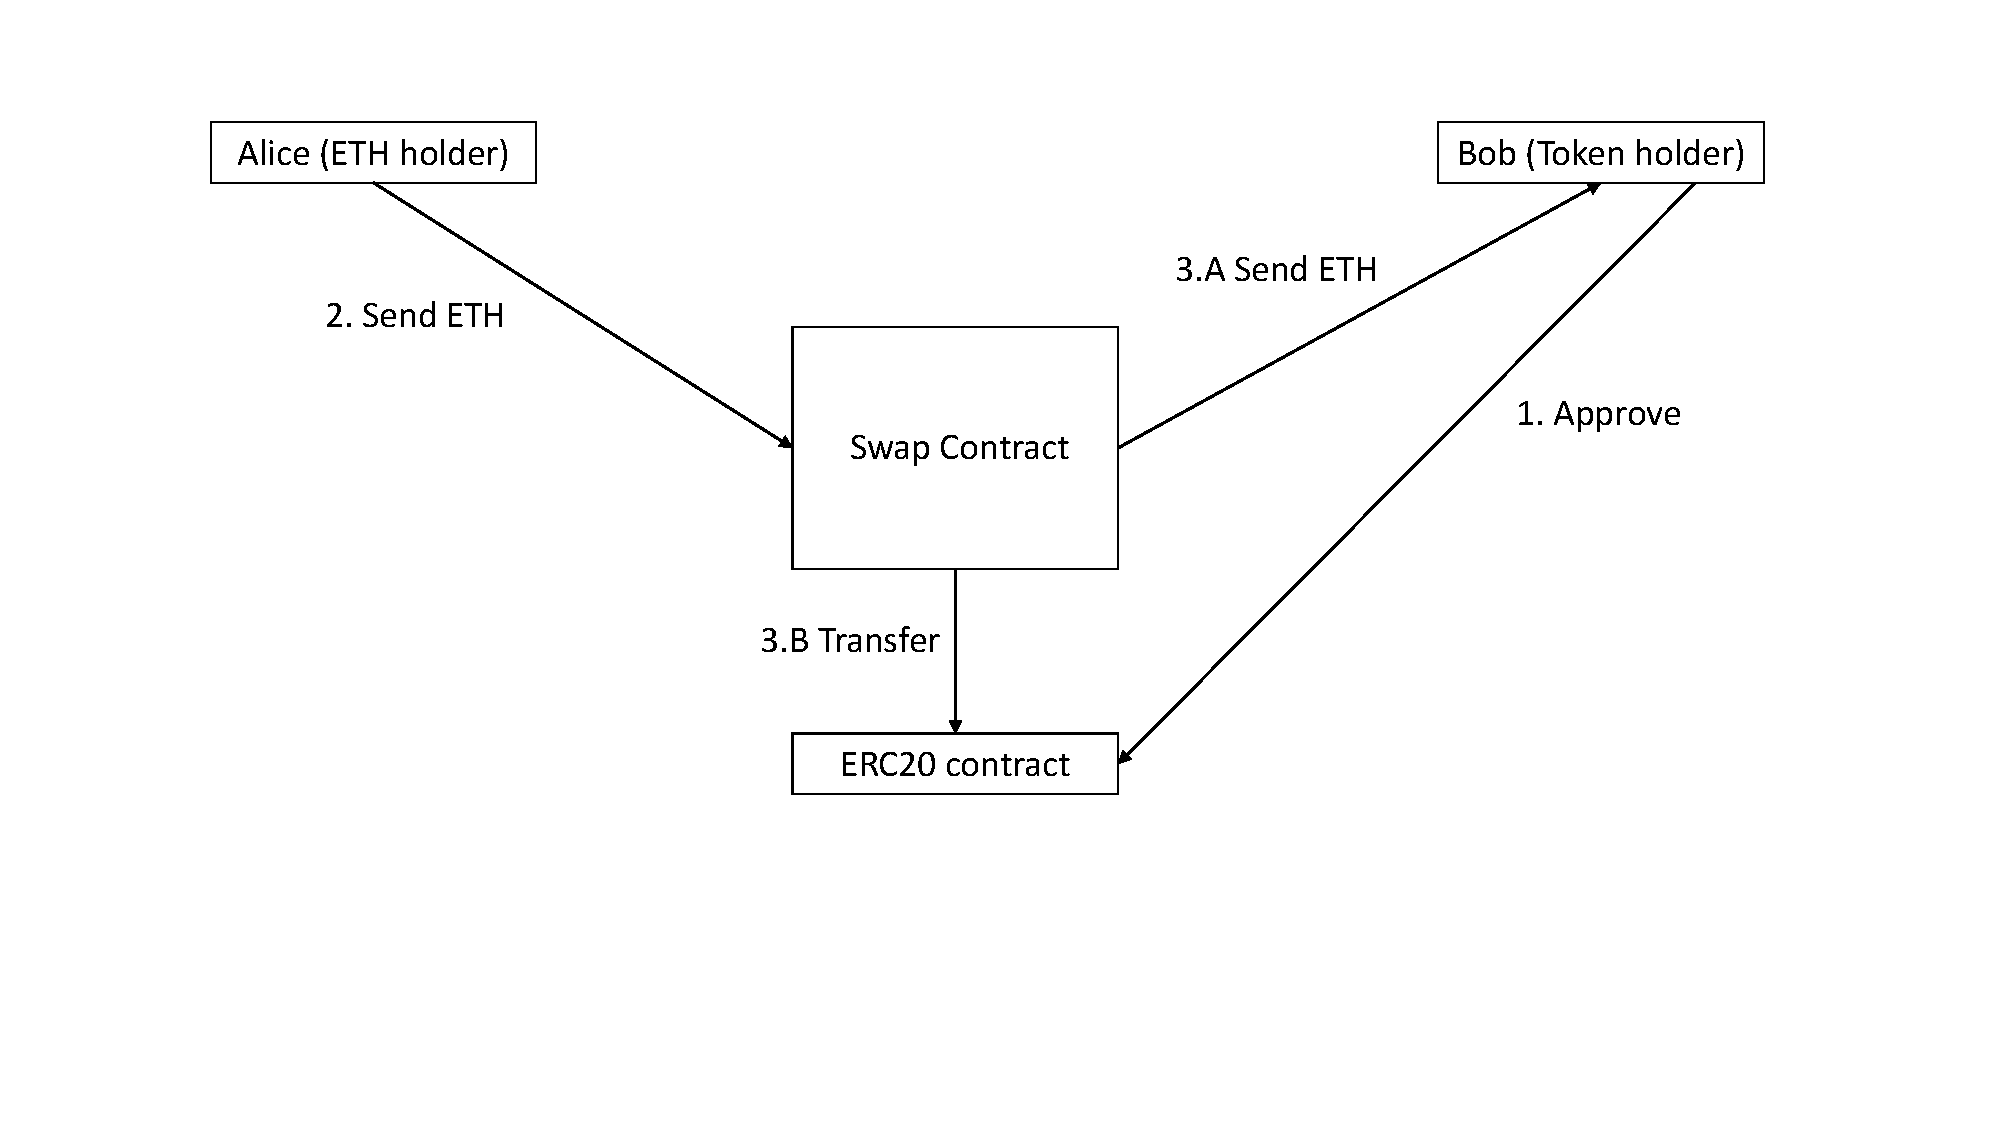
\includegraphics[width=1\textwidth]{approve}
%\caption{ETH to ERC20 with approve}
%\label{fig:withapprove}
%\vspace{-10pt}
%\end{figure}
%
%\begin{figure}[h!]
%\centering
%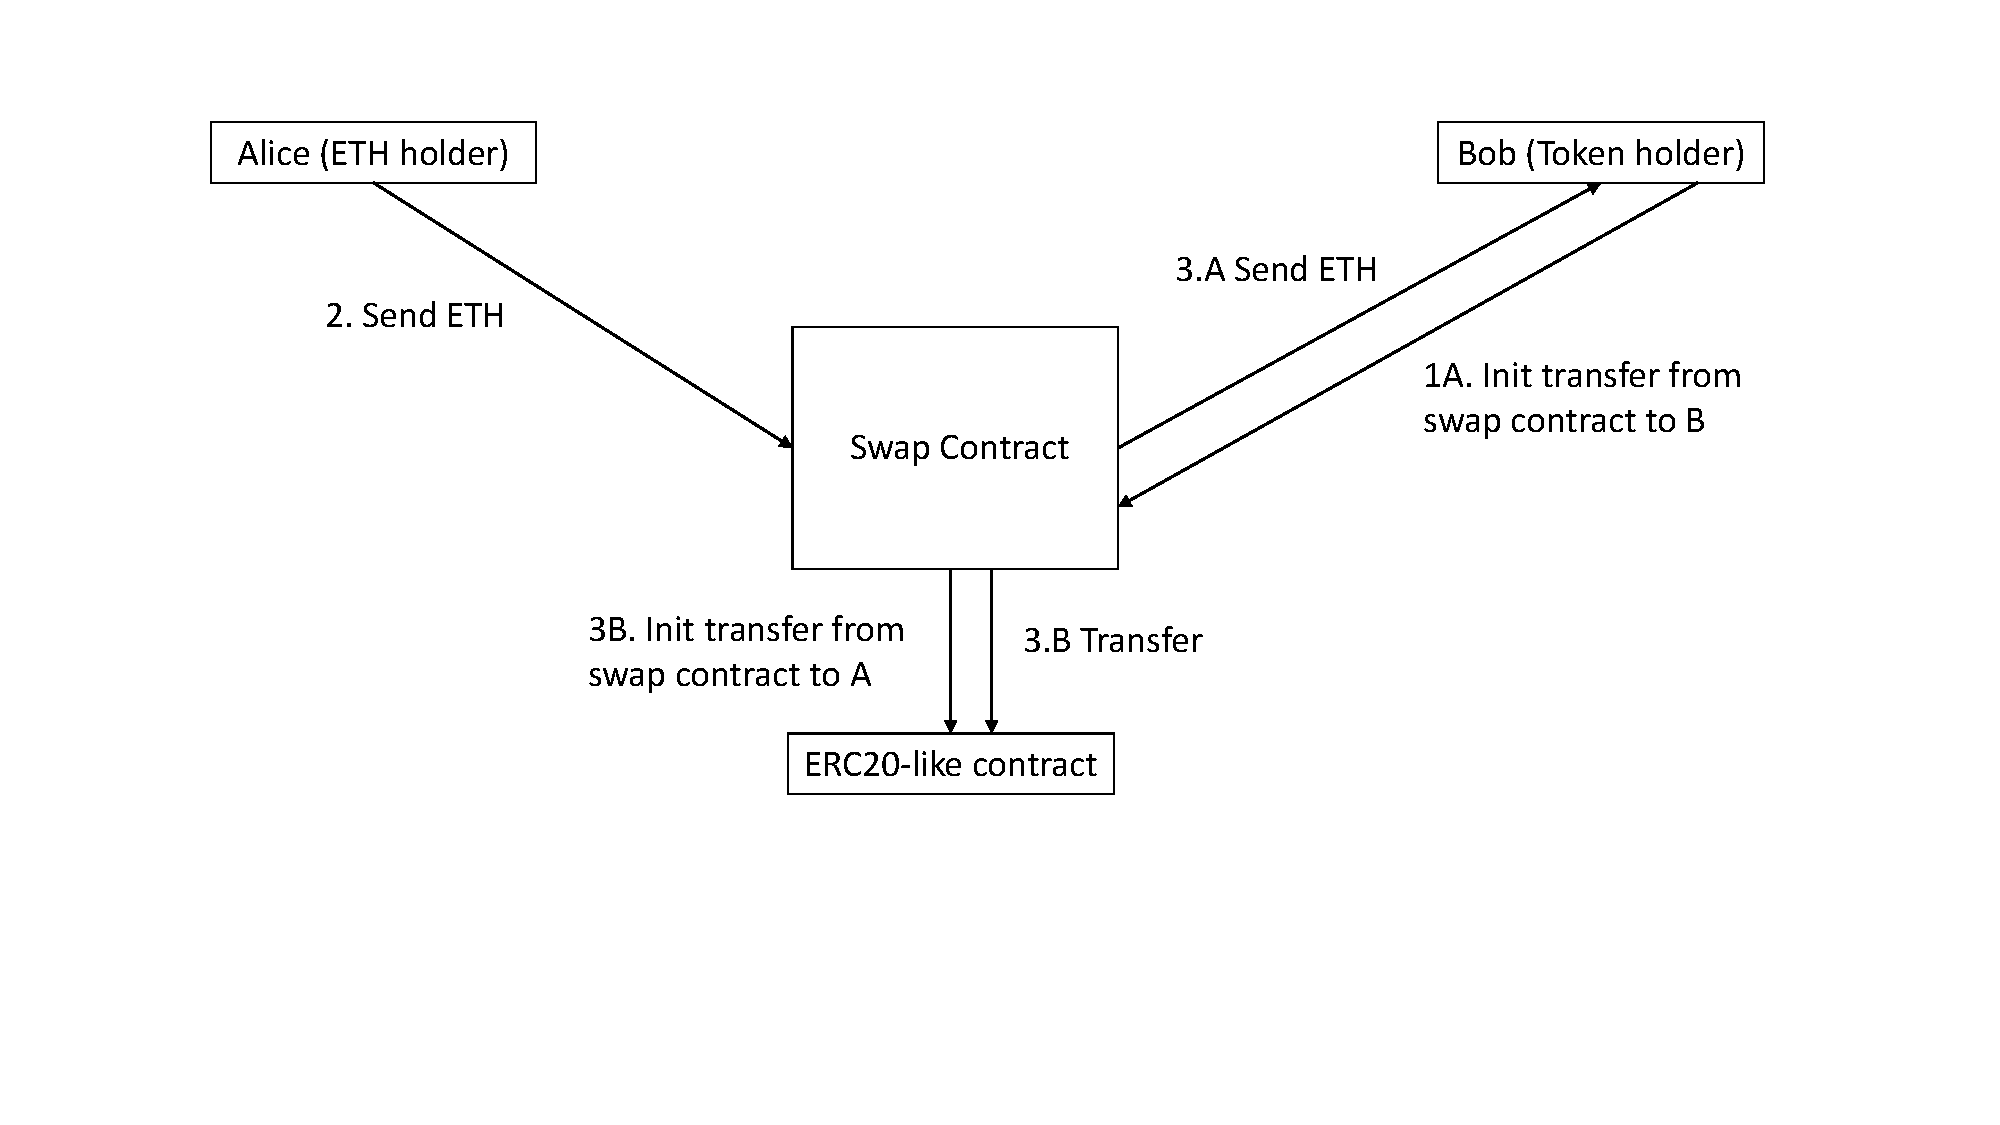
\includegraphics[width=1\textwidth]{withoutapprove}
%\caption{ETH to ERC20-like without approve}
%\label{fig:withoutapprove}
%\vspace{-10pt}
%\end{figure}
%
%\begin{figure}[h!]
%	\centering
%	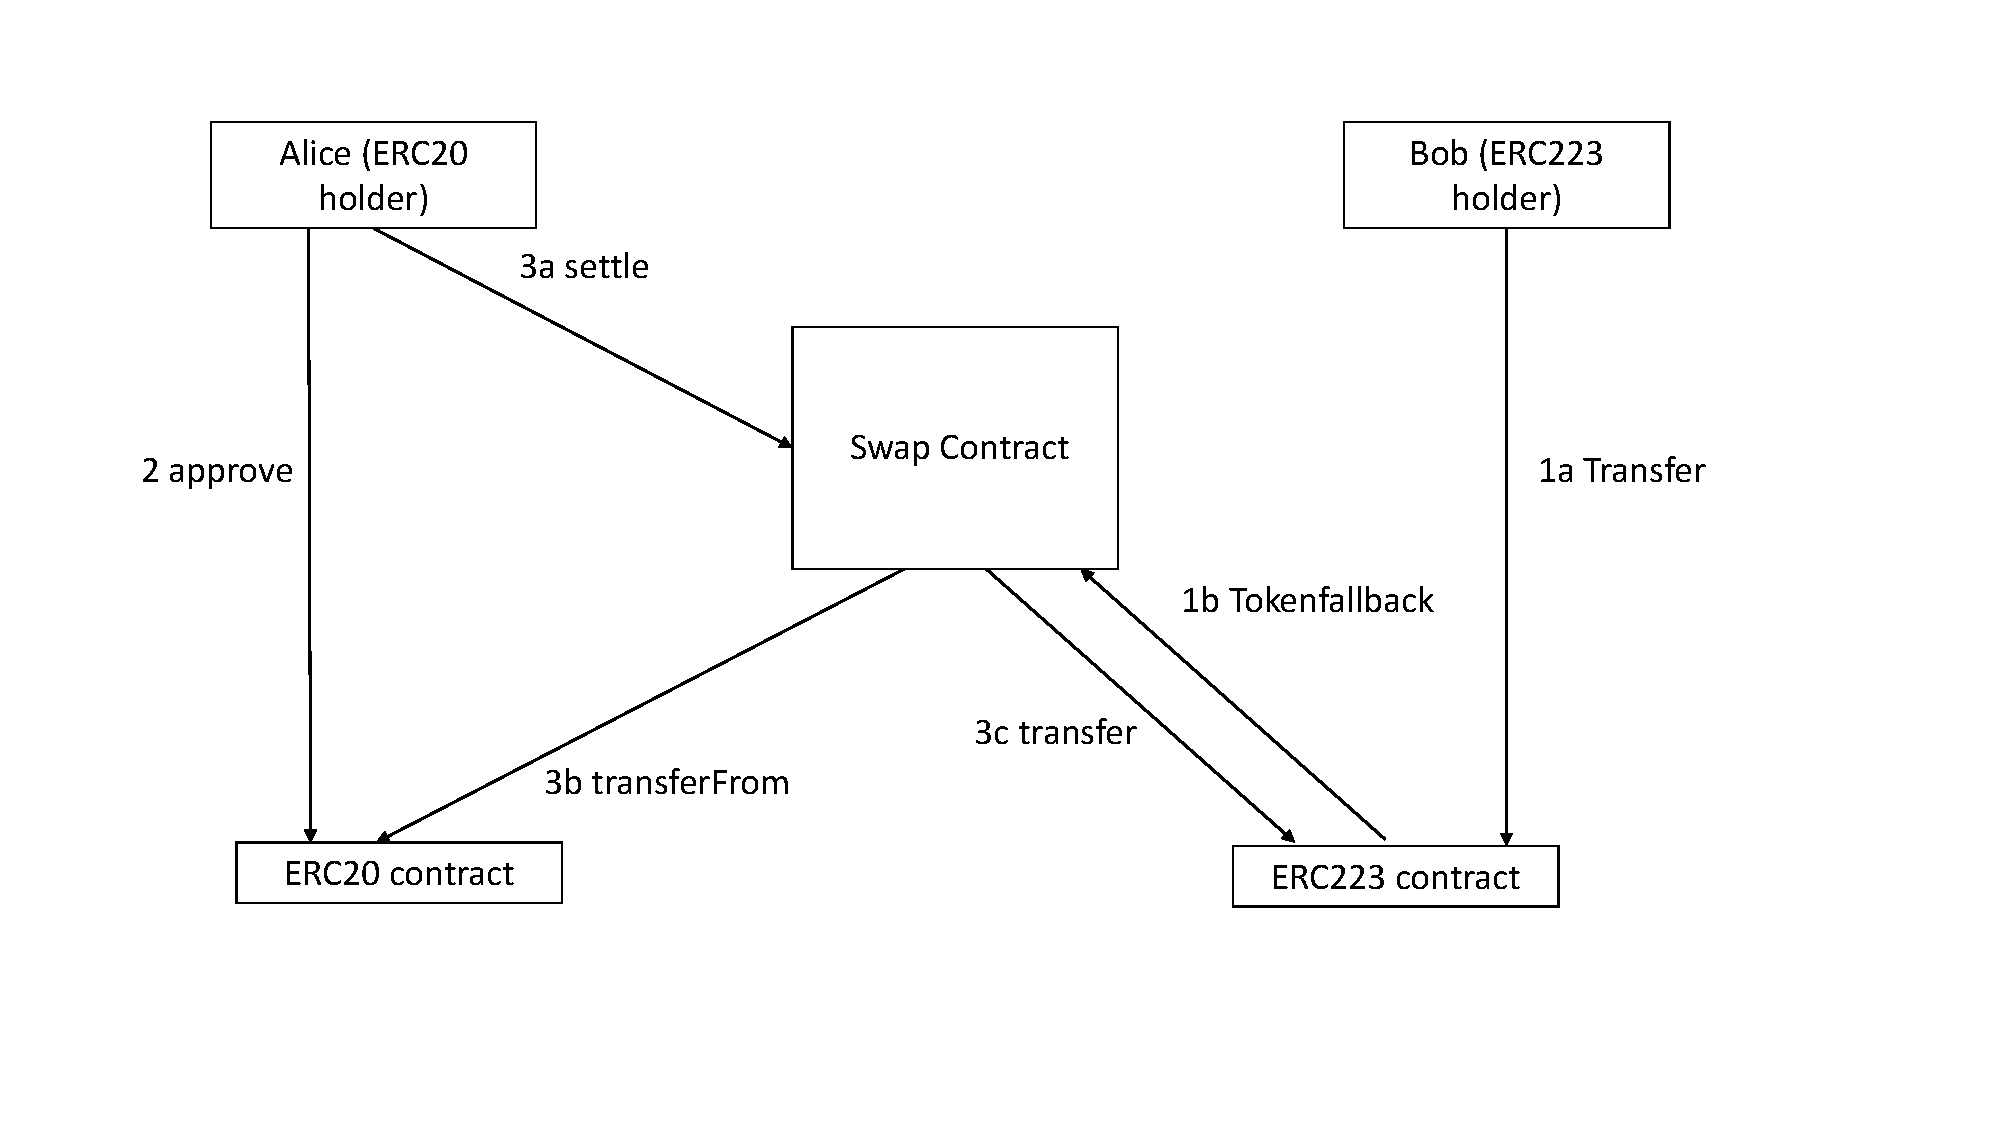
\includegraphics[width=1\textwidth]{ERC20toERC223}
%	\caption{ERC20 to ERC223}
%	\label{fig:ERC20toERC223}
%	\vspace{-10pt}
%\end{figure}
%
%\begin{figure}[h!]
%	\centering
%	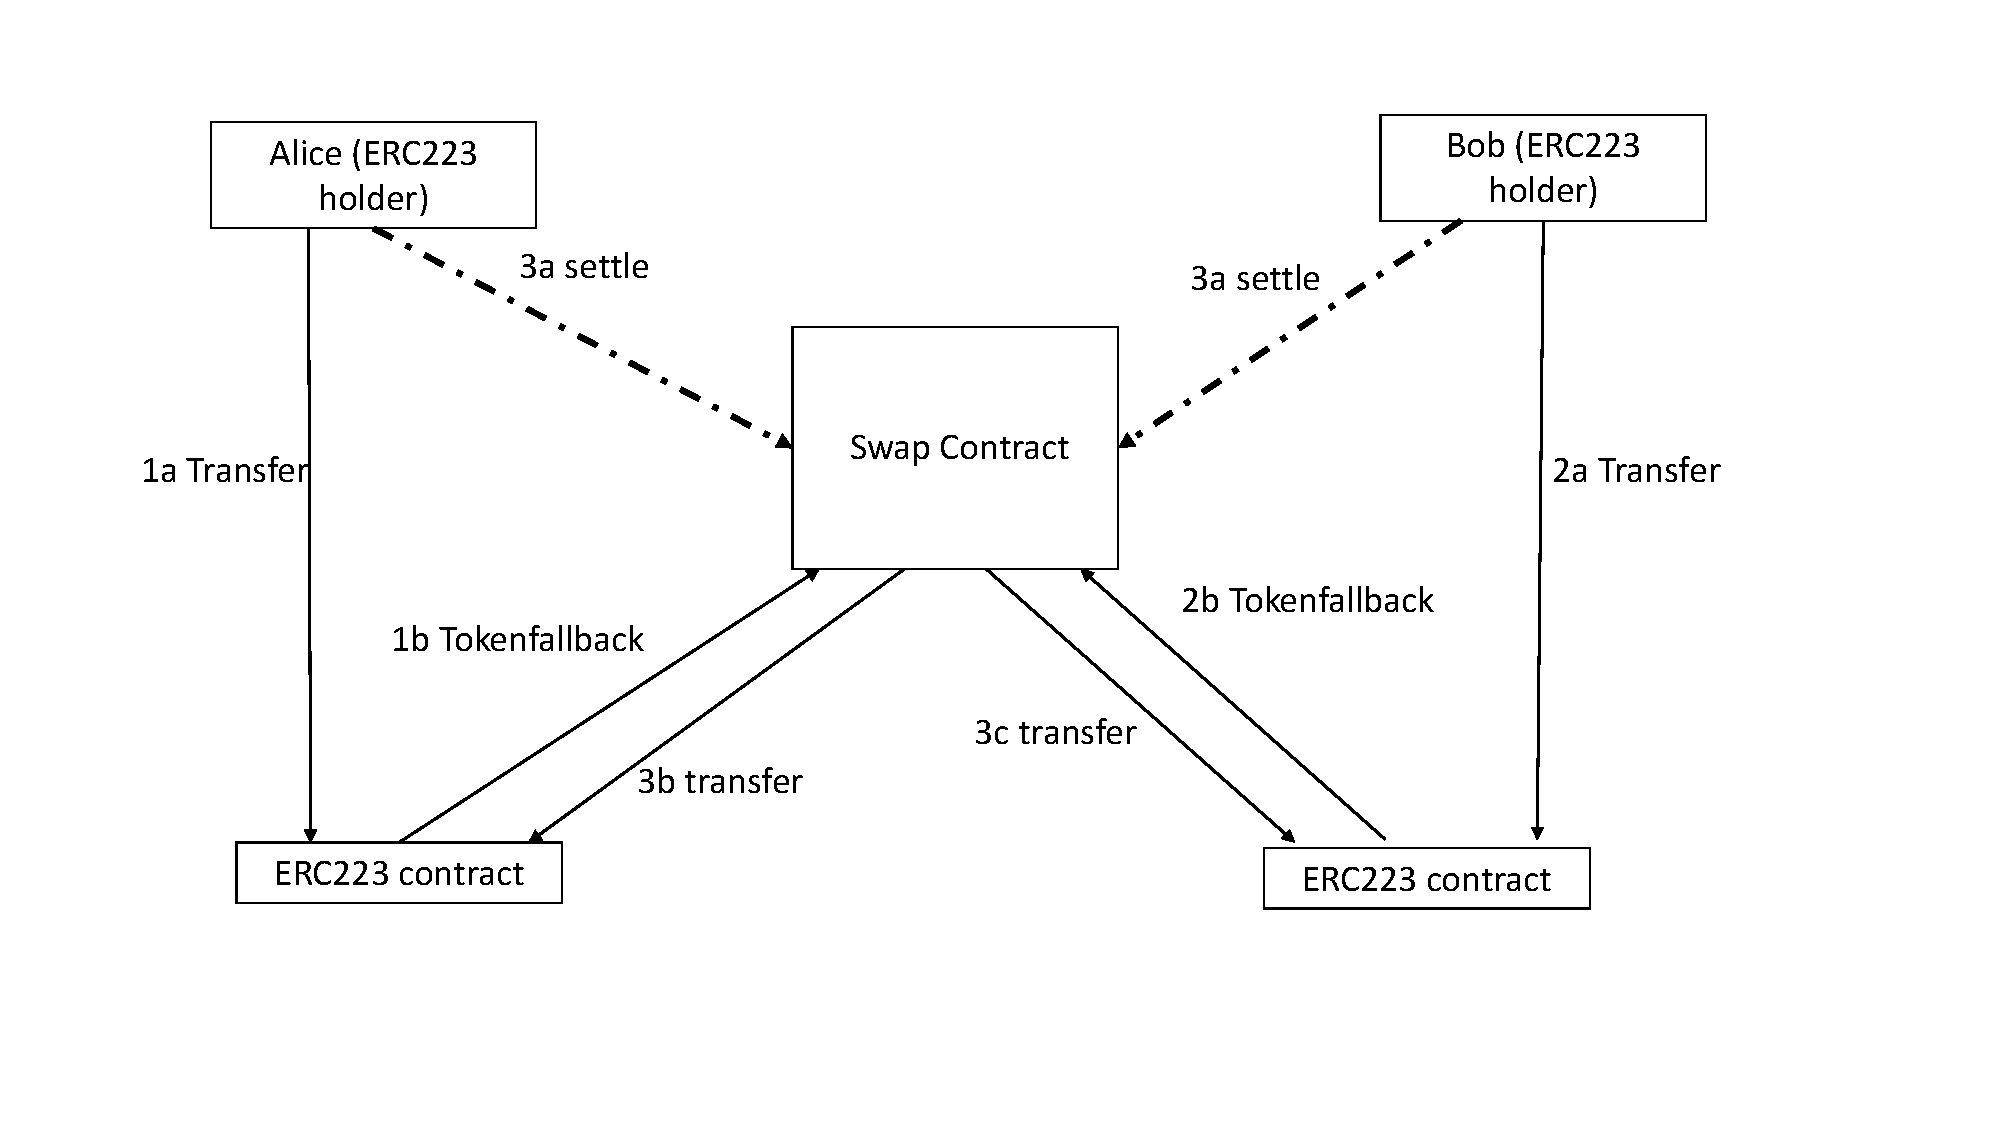
\includegraphics[width=1\textwidth]{ERC223toERC223}
%	\caption{ERC223 to ERC223}
%	\label{fig:ERC223toERC223}
%	\vspace{-10pt}
%\end{figure}
%
%\begin{figure}[h!]
%	\centering
%	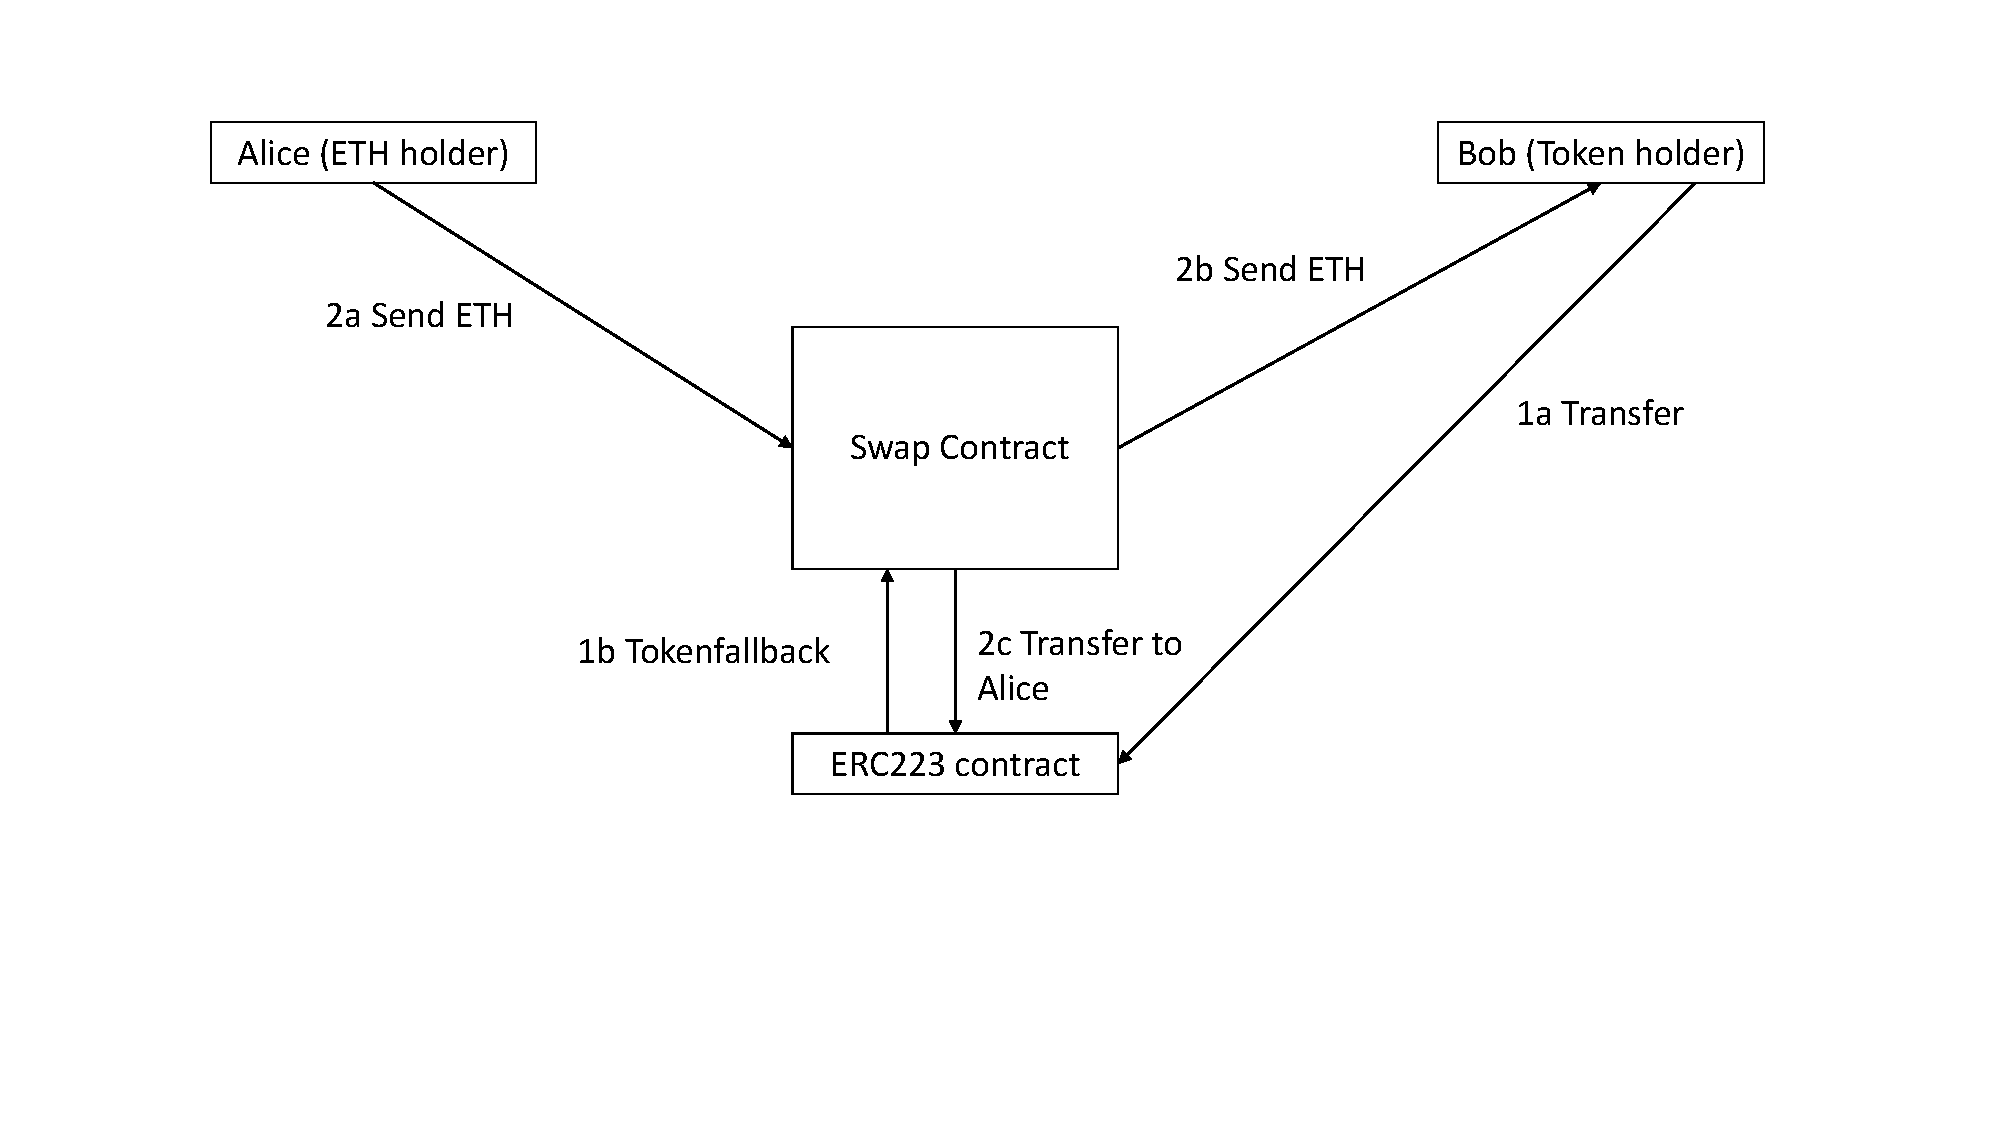
\includegraphics[width=1\textwidth]{ETHtoERC223}
%	\caption{ETH to ERC223}
%	\label{fig:ETHtoERC223}
%	\vspace{-10pt}
%\end{figure}
%
%\section{Comparison of Token Standards}
%\subsection{ERC721}
%non-fungible, ERC20 compatible
%\subsection{ERC223}
%ERC20 has the problem of "non-recovarable" coins
%ERC20 needs to execute two functions to transfer coins: approve and transferFrom. ERC223 consumes half the amount of gas than the amount needed to transfer an ERC20 token.
%ERC223 offers 3 improvements:
%\begin{itemize}
%  \item no lost tokens
%  \item reject non-supported tokens
%  \item energy saving
%\end{itemize}
%
%tokenFallback: the receiving contract has a chance to do some work.
%\subsection{ERC777}

\section{Background}
ERC stands for Ethereum Request for Comment~\cite{comparison}. The emergence of ERC20 tokens in 2015 made the token creation much easier. There are six main functions in the interface~\cite{ERC20}: totalSupply, balanceOf, transfer, transferFrom, approve and allowance. Transfer moves a certain amount of tokens to a given adress. TransferFrom transfers tokens from one token contract to another. Approve functions specifies the amount of tokens that can be withdrawn from an account. There is a significant shortcoming of current ERC20 implementation: a party may send tokens to a contract that it doesn't intend to. In this case, the party won't be able get its tokens back.

ERC223 addresses the aforementioned problem that ERC20 has~\cite{ERC223}. ERC223's transfer function prevents lost tokens, as it prevents transferring tokens to contracts which are not expecting them. ERC223 token transfer works similar to the ETH transactions. If a party tries to transfer tokes to a non-receiver contract, an exception will be thrown. ERC223's transfer function is more efficient than ERC20's approve and transferFrom, as it consumes less gas.

\section{Atomic swaps with different settings}
Atomic swaps can be realized using different kinds of tokens and there can be different variations depending on the function calls used or collateralization. Table~\ref{Table:Comparison of different swaps} illustrates the possible settings and compares the amount of transactions required for each case. %The involving parties in the swap are named as maker and taker in accordance with the financial terminology, where maker is the party that provides the token or ETH and taker is the party that wants to buy token or ETH from the maker.
The class determines certain characteristics of the swap. Approve means that the approve function in the token interface is used and without approve corresponds to the opposite case. Both approve and without approve class type swaps are not collateralized due to the properties of the ERC20 token. Hybrid refers to the  case where one party collateralizes its assets and the other doesn't.

\begin{table}[h!]
\footnotesize
\centering
%\Huge
%\resizebox{\columnwidth}{!}{%
\begin{tabular}{ |c|c|c|c|c|c| }
  \hline
   maker & taker & class & order transactions  & account (onetime)  \\
   & & &(margin) &  transactions (fixed) \\ \hline
   ERC20 & ETH & approve & 2 & 4 \\ \hline
   ERC20 & ERC20 & approve & 2 & 5 \\ \hline
   ERC20-like & ETH & w/o approve & 2 & 4 \\ \hline
   ERC20-like & ERC20-like & w/o approve & 2 & 5 \\ \hline
   ERC223 & ETH & hybrid & 2 & 4\\ \hline
   ERC20 & ETH & collateralized & &\\ \hline
   ERC20 & ETH & partially collateralized & &\\ \hline
   ERC20 & ERC223 & hybrid & 2 & 5 \\ \hline
   ERC223 & ERC223 & collateralized & 3 & 4\\ \hline
\end{tabular}
\caption {swaps}
%}
\end{table}\label{Table:Comparison of different swaps}
\textbf{ERC20 to ETH:}  Somebody deploys the swap contract. For each atomic swap between two parties, somebody (who may or may not be one of the transacting parties) initiates a swap object within the swap contract. Token holder calls approve on the ERC20 contract with the swap contract as the target/allowance holder/spender. The token holder may approve the swap contract for multiple transactions by setting an allowance greater than necessary for one swap. The holder of the ETH calls a settle function on the swap contract, sending their ETH along with it. This triggers the swap and the swap contract calls transferFrom on the ERC20 contract, transferring the tokens from the token holder to the ETH holder. The swap contract at this stage also sends the ETH to the token holder. The atomic swap is now complete. Deploying the swap contract and approving on the ERC20 contract are considered as the fixed transactions as they do not need to be performed for every swap. The swap initialization and calling of the settle function, both within the swap contract, must be carried out for every swap. When taken with the fixed cost transactions, an atomic swap takes up to four transactions total.

\textbf{ERC20 to ERC20:} All the transactions described in the setting for ETH to ERC20 swap are also observed in this case. In addition to those, for the fixed transactions, we have 5 in total as the other token holder should also approve the amount of tokens to be spent.

\textbf{ERC20-like to ETH:} For this setting, the approve function in the ERC20 interface is not used. Similar to the ETH to ERC20 case, we have 4 transactions in total, that consists of deploying the swap contract, initializing the swap object, calling the settle function to send ETH and transfer of tokens to the swap contract. Deploying the swap contract and transferring the tokens to swap contract are considered as the fixed transactions, as a party can transfer more tokens than a single swap requires, which allows the involving parties to perform several swaps.

\textbf{ERC20-like to ERC20-like:} The token standard used in this case is defined as ERC20-like, as the approve function that is defined in the ERC20 interface is not utilized. Apart from the 2 fixed transactions (deploying the swap contract and transferring the tokens to the swap contract), there are 3 more transactions in this case. The approve function is replaced by a function that consists of two parts: token holder initiates transfer from swap contract and the transfer from the token contract takes place. This should be performed by both parties. And the last one is the settle function that finalizes the swap.

\textbf{ERC223 to ETH:} The ERC223 interface allows the parties to collateralize the tokens. However, the ETH is not collateralized. This case is defined as hybrid. In addition to the fixed transactions, there are two more transactions that needs to be performed at each swap. First transaction calls the transfer and the tokenfallback to let the swap contract know about the swap. Second transaction is the settle function where the ETH owner sends ETH to the swap contract and the swap contract sends the ETH to the token owner. As a last step of the transaction function, swap contract triggers the token contract to send the tokens to the ETH holder.

\textbf{ERC20 to ERC223:} Deploying the swap contract and transferring the tokens to the swap contract are counted as fixed transactions. In addition to them, settling the swap (sending the ETH to the token owner and sending the tokens to the ETH owner) and the tokenFallback function that acts similar to the approve function in ERC20 are the order transactions as they have to be performed every time a swap occurs. The class of the swap is defined as hybrid, since the ERC223 tokens are collateralized, while the ERC20 tokens are not.

\textbf{ERC223 to ERC223:} Once the swap is initialized, both parties must invoke the transfer function of their corresponding token contracts in order to transfer the tokens to the swap contract. Settlement can then be triggered by either party and the swap is executed. This type of swap is fully collateralized and takes 4 transactions total. Three of the transactions must occur with each swap, while the initialization of the swap contract need only be carried out once. Unlike with an ERC20 swap, it is not straightforward to escrow multiple swaps worth of ERC223 tokens with a single transaction.

\section{Conclusion}
Atomic swaps can be realized in different settings.
